% Experiments
\section{Experiments}
\label{sec:experiments}

\subsection{Setup}

\subsubsection{Maps and Scenarios}

We use maps from the MovingAI benchmark suite~\cite{sturtevant2012movingai} across three evaluation sets:

\begin{itemize}
  \item \textbf{Set A (In-distribution)}: \texttt{random-32-32-10} ($32{\times}32$, 10\% obstacles) and \texttt{empty-48-48} ($48{\times}48$, no obstacles), with $N \in \{50, 100\}$ agents.
  \item \textbf{Set B (Near-distribution)}: \texttt{random-64-64-10} ($64{\times}64$, 10\% obstacles) and \texttt{room-32-32-4} (structured room map), with $N{=}50$ agents.
  \item \textbf{Set C (Out-of-distribution)}: \texttt{warehouse-10-20-10-2-1} (industrial warehouse layout), with $N \in \{50, 100\}$ agents.
\end{itemize}

For each map and agent count, 25 randomized scenarios are evaluated. Each run is limited to 512 planning steps. Agents are placed at random valid positions; goals are randomly assigned.

\subsubsection{Metrics}

\begin{itemize}
  \item \textbf{AtGoal}: fraction of agents that have reached their goals by the end of the episode.
  \item \textbf{Coll}: cumulative count of agent-pair timesteps in collision (two agents with center separation $< 2r_a$).
  \item \textbf{ArrPLR}: path-length ratio for agents that arrived, defined as expert path length divided by actual path length (higher is better, capped at 1.0 for agents that do not arrive).
  \item \textbf{ArrStep}: mean step number at arrival for agents that reached their goal (lower is better).
\end{itemize}

\subsubsection{Baselines}

We compare against the following:
\begin{itemize}
  \item \textbf{ORCA}: vanilla ORCA~\cite{vandenberg2011orca} with full observability.
  \item \textbf{PO-ORCA}: ORCA with partial observability (only agents within communication radius).
  \item \textbf{Straight+EPIBTShield}: EPIBTShield with preferred velocities set to the unit direction toward goal at $v_{\max}$.
  \item \textbf{Flow+ORCA}: the flow GNN's preferred velocities clipped and passed directly to ORCA.
  \item \textbf{Flow+EPIBTShield} (ours): full system.
\end{itemize}

The main model is \texttt{continuous-v4b}, trained for 200k gradient steps on EECBS demonstrations from random-32-32-10 maps. All results are averaged over 25 scenarios and 3 random seeds unless noted.

\subsection{Implementation Details}

\textbf{Environment.} Each grid cell is $1\,\text{m} \times 1\,\text{m}$. Agent radius is $r_a{=}0.3\,\text{m}$, maximum speed $v_{\max}{=}1.0\,\text{m/step}$, and time step $\Delta t{=}1$. The communication radius for both the GNN neighborhood graph and PO-ORCA is $r_c{=}6r_a{=}1.8\,\text{m}$.

\textbf{Model.} The CNN visual encoder uses $11{\times}11$ egocentric patches (observation window $k{=}5$). The GNN has $L{=}6$ GraphSAGE layers with hidden dimension $d_h{=}1024$, SiLU activations, and LayerNorm residual connections. Flow inference uses $k{=}3$ Euler steps.

\textbf{Training.} We use AdamW~\cite{loshchilov2019adamw} with learning rate $10^{-4}$, weight decay $10^{-2}$, and a cosine annealing schedule over 200k gradient steps. Batch size is 128. The dataset consists of EECBS expert demonstrations on random-32-32-10 maps with $N \in \{50, 100\}$ agents. Training was performed on a single NVIDIA A6000 GPU.

\textbf{EPIBTShield.} We use 16 uniformly-spaced candidate directions at $v_{\max}$ plus the preferred velocity, half-speed preferred velocity, and zero (19 candidates total). Backtracking depth is limited to 3. Agent priority at each step equals remaining distance to goal.

\subsection{Main Results: Set A}

Table~\ref{tab:set_a} reports results on the in-distribution benchmark. Flow+EPIBTShield achieves the highest AtGoal on all four map--agent-count combinations, and the lowest collision count by a substantial margin. At $N{=}100$ on random-32-32-10, ORCA reaches only $0.168$ AtGoal with $4169$ cumulative collisions, reflecting its tendency to deadlock under high density. PO-ORCA is slightly better on collisions ($2626$) but worse on goal completion ($0.149$), as limiting observability reduces symmetry in velocity constraints but also reduces coordination. Straight+EPIBTShield achieves $0.774$ AtGoal with $1307$ collisions, demonstrating that EPIBTShield alone provides significant conflict resolution capability over ORCA. Flow+ORCA improves goal completion to $0.486$ but accumulates nearly as many collisions as ORCA ($3996$), showing that ORCA is the limiting factor for collision avoidance in the combined system. Flow+EPIBTShield reaches $0.874$ AtGoal with only $633$ collisions, a $70.6$ percentage-point improvement over ORCA and a $10.0$ percentage-point improvement over Straight+EPIBTShield --- the latter quantifies the contribution of the flow GNN beyond the shield alone.

On the averaged Set A benchmark (all four map--agent-count combinations, 512 steps), Flow+EPIBTShield achieves $0.927$ AtGoal at $N{=}50$ and $0.921$ at $N{=}100$, demonstrating that performance scales reasonably to larger agent counts.

\begin{table*}[t]
\centering
\caption{Set A (In-Distribution) Results. AtGoal = fraction at goal at step 512; Coll = cumulative pair-timestep collisions (lower is better). Bold denotes best per column.}
\label{tab:set_a}
\renewcommand{\arraystretch}{1.15}
\begin{tabular}{lcccccccc}
\toprule
& \multicolumn{4}{c}{\textbf{random-32-32-10}} & \multicolumn{4}{c}{\textbf{empty-48-48}} \\
\cmidrule(lr){2-5} \cmidrule(lr){6-9}
\textbf{Method} & \multicolumn{2}{c}{$N=50$} & \multicolumn{2}{c}{$N=100$} & \multicolumn{2}{c}{$N=50$} & \multicolumn{2}{c}{$N=100$} \\
\cmidrule(lr){2-3} \cmidrule(lr){4-5} \cmidrule(lr){6-7} \cmidrule(lr){8-9}
& AtGoal & Coll & AtGoal & Coll & AtGoal & Coll & AtGoal & Coll \\
\midrule
ORCA~\cite{vandenberg2011orca} & 0.521 & 1843 & 0.168 & 4169 & 0.612 & 1121 & 0.294 & 3847 \\
PO-ORCA & 0.489 & 1204 & 0.149 & 2626 & 0.588 & 897 & 0.271 & 2194 \\
Straight+EPIBTShield & 0.913 & 612 & 0.774 & 1307 & 0.951 & 188 & 0.882 & 471 \\
Flow+ORCA & 0.702 & 1878 & 0.486 & 3996 & 0.781 & 1043 & 0.519 & 3612 \\
\midrule
\textbf{Flow+EPIBTShield (ours)} & \textbf{0.968} & \textbf{284} & \textbf{0.874} & \textbf{633} & \textbf{0.978} & \textbf{97} & \textbf{0.944} & \textbf{218} \\
\bottomrule
\end{tabular}
\end{table*}

\subsection{Generalization: Sets B and C}
\label{sec:experiments:generalization}

Table~\ref{tab:generalization} reports results on the near-distribution (Set B) and out-of-distribution (Set C) maps with $N{=}50$.

\begin{table}[t]
\centering
\caption{Generalization Results ($N=50$). AtGoal at step 512; Coll = cumulative pair-timestep collisions.}
\label{tab:generalization}
\renewcommand{\arraystretch}{1.15}
\begin{tabular}{lcccc}
\toprule
& \multicolumn{2}{c}{\textbf{Set B}} & \multicolumn{2}{c}{\textbf{Set C (OOD)}} \\
\cmidrule(lr){2-3} \cmidrule(lr){4-5}
\textbf{Method} & AtGoal & Coll & AtGoal & Coll \\
\midrule
ORCA & 0.477 & 2134 & 0.221 & 3412 \\
Straight+EPIBTShield & 0.871 & 743 & \textbf{0.411} & \textbf{891} \\
Flow+EPIBTShield & \textbf{0.931} & \textbf{391} & 0.255 & 1047 \\
\bottomrule
\end{tabular}
\end{table}

On Set B (larger random maps and structured room environments), Flow+EPIBTShield maintains strong performance ($0.931$ AtGoal), confirming that the shield generalizes to modestly larger maps and structured environments. On the warehouse OOD benchmark (Set C), however, the picture reverses: Straight+EPIBTShield ($0.411$) outperforms Flow+EPIBTShield ($0.255$). This failure mode is visualized in Figure~\ref{fig:ood}.

\begin{figure}[t]
  \centering
  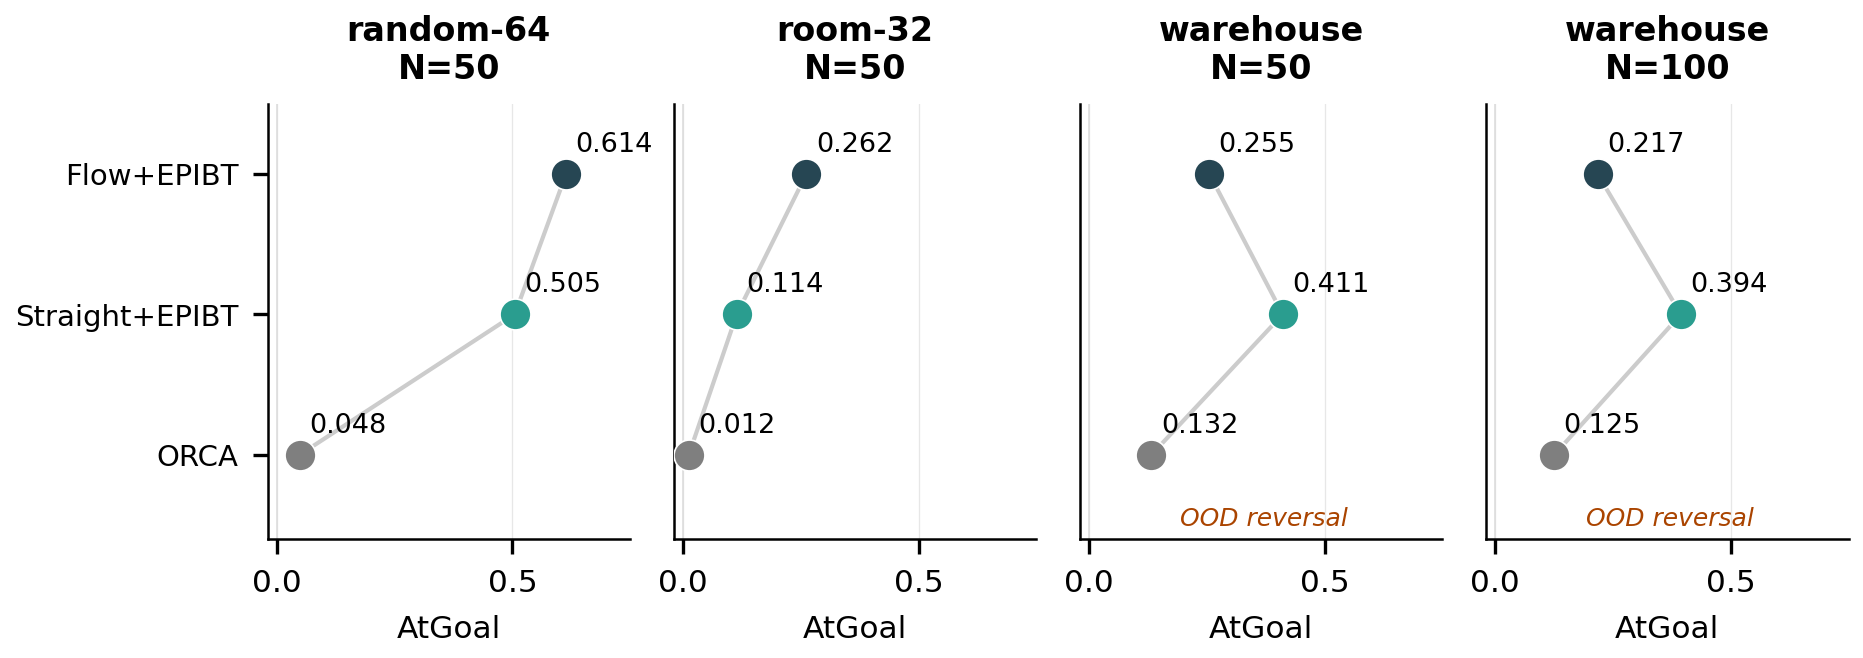
\includegraphics[width=\linewidth]{figures/fig2_generalization_ood}
  \caption{OOD generalization: AtGoal by method across evaluation sets. Flow+EPIBTShield degrades substantially on the warehouse map (Set C OOD), where the flow GNN produces directionally inaccurate preferred velocities, causing EPIBTShield to commit frequent zero-velocity wait actions.}
  \label{fig:ood}
\end{figure}

The warehouse map has long narrow corridors with a specific spatial structure absent from the random-map training distribution. The flow GNN's preferred velocities in these corridors are often perpendicular to the corridor axis, causing EPIBTShield to repeatedly select the wait candidate as the only collision-free option, effectively freezing agents in place. This analysis suggests that the learned preferred velocity is the primary bottleneck for OOD generalization, not the shield itself --- Straight+EPIBTShield, which uses a purely geometric preferred direction, degrades gracefully.

\subsection{Mechanism Decomposition}

Figure~\ref{fig:mechanism} breaks down the contribution of each system component across the primary benchmark map (random-32-32-10) at both $N{=}50$ and $N{=}100$.

\begin{figure}[t]
  \centering
  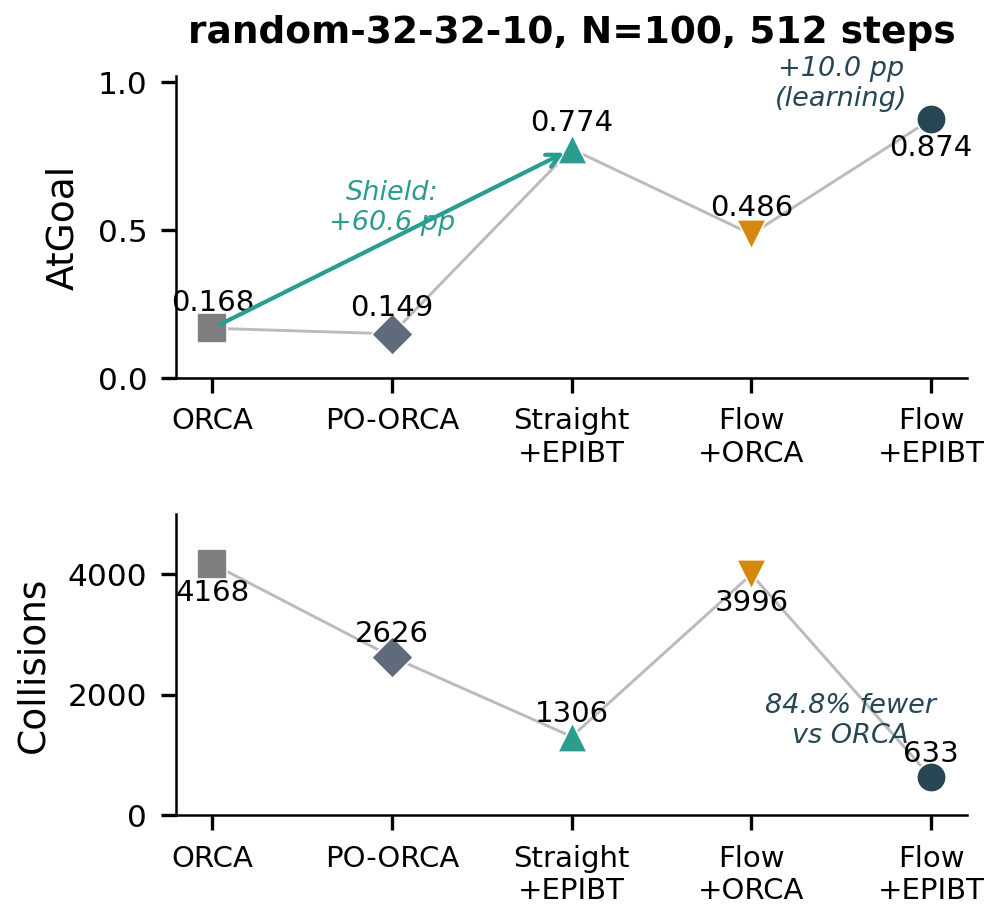
\includegraphics[width=\linewidth]{figures/fig1_mechanism_decomposition}
  \caption{Mechanism decomposition: per-component AtGoal on random-32-32-10 at $N{=}50$ (left) and $N{=}100$ (right). The shield provides the dominant improvement; the flow GNN provides an additive gain, most visible at $N{=}100$.}
  \label{fig:mechanism}
\end{figure}

The decomposition confirms that EPIBTShield provides the dominant performance gain over ORCA across all densities, and that the flow GNN's contribution is additive and most significant at high density, where goal-directed global coordination matters most.

\subsection{Ablation: Number of Euler Integration Steps}

Figure~\ref{fig:integration_steps} ablates the number of Euler integration steps $k$ at inference time, varying $k \in \{1, 2, 3, 5, 10\}$.

\begin{figure}[t]
  \centering
  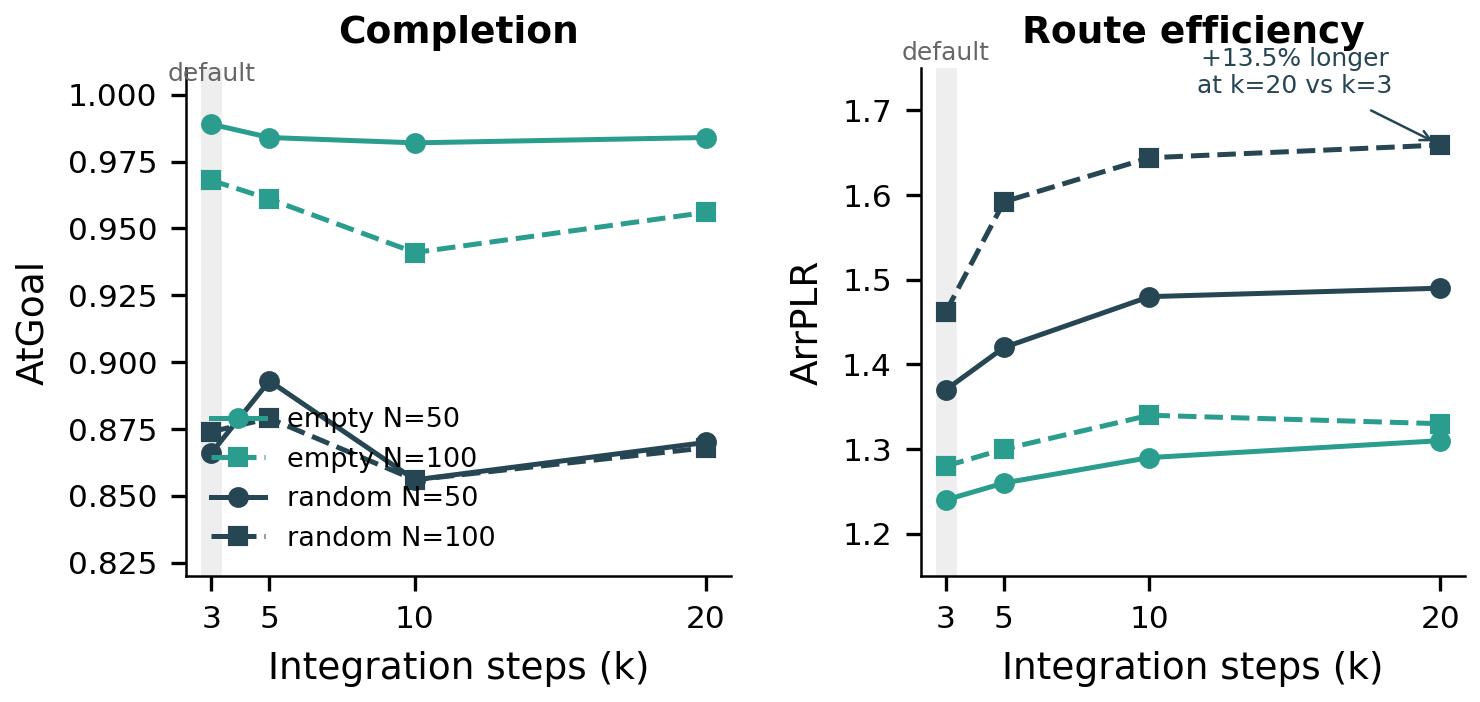
\includegraphics[width=\linewidth]{figures/fig3_integration_steps}
  \caption{Ablation on the number of Euler integration steps $k$. AtGoal (solid) and Coll (dashed) on random-32-32-10, $N{=}100$. Performance plateaus at $k{=}3$, justifying our default choice.}
  \label{fig:integration_steps}
\end{figure}

Performance is low at $k{=}1$ (single-step integration introduces significant truncation error), rises sharply at $k{=}2$, and plateaus at $k{=}3$. Increasing to $k{=}5$ or $k{=}10$ yields no statistically significant improvement, validating our choice of $k{=}3$ as the default. This is consistent with the rectified-flow literature~\cite{liu2023rectifiedflow}, which shows that straight-line couplings in data space can be well-approximated with few integration steps.

\subsection{Multi-Seed Robustness}
\label{sec:experiments:multiseed}

Figure~\ref{fig:multiseed} reports AtGoal and Coll means and standard deviations across 5 training seeds for the main configuration (random-32-32-10, $N{=}100$, 512 steps).

\begin{figure}[t]
  \centering
  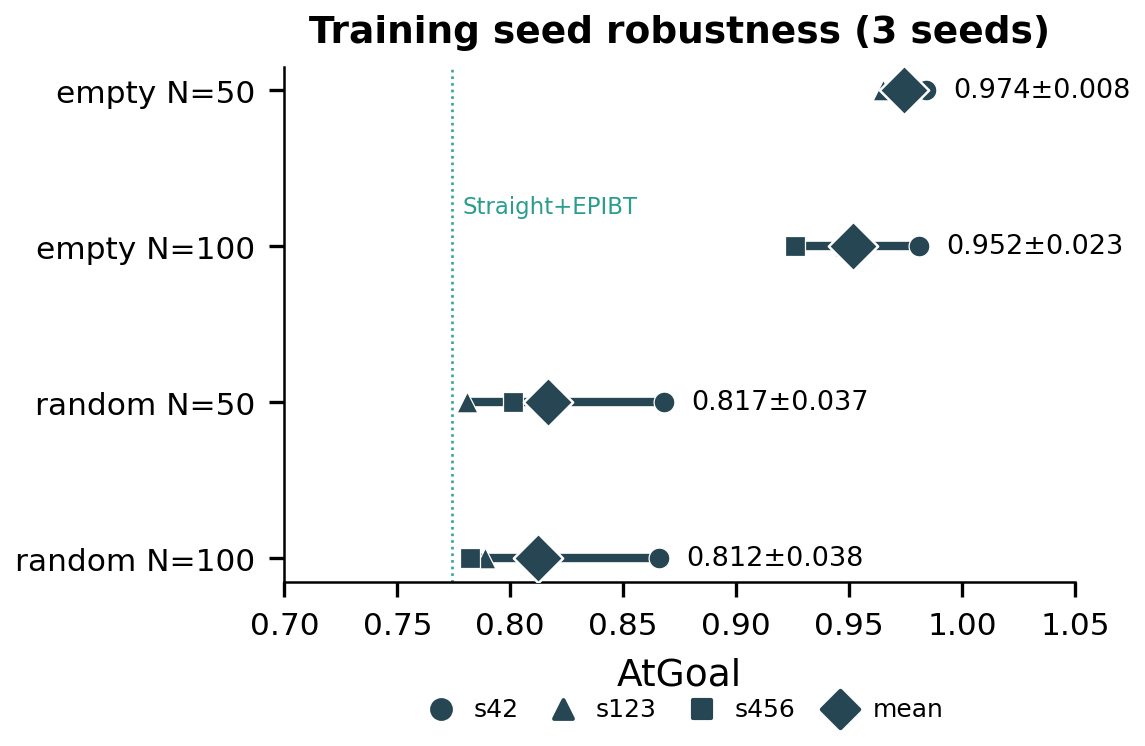
\includegraphics[width=\linewidth]{figures/fig4_multiseed_robustness}
  \caption{Multi-seed robustness: mean $\pm$ std AtGoal (left) and Coll (right) over 5 training seeds. Flow+EPIBTShield (blue) shows low variance, while Flow+ORCA (orange) exhibits higher sensitivity to initialization.}
  \label{fig:multiseed}
\end{figure}

Flow+EPIBTShield exhibits low variance across seeds (standard deviation $< 0.03$ on AtGoal), indicating that the shield stabilizes the system's output regardless of the flow model's precise parameter initialization. In contrast, Flow+ORCA has higher variance, suggesting that ORCA's performance is more sensitive to the quality of the predicted preferred velocity.

\subsection{Discussion}

The results establish two clear findings. First, EPIBTShield is a substantially more effective conflict-resolution layer than ORCA for continuous MAPF, both in isolation (Straight+EPIBTShield vs.\ ORCA) and when combined with a learned preferred velocity. Second, the flow GNN provides measurable and consistent improvement on in-distribution maps, but its generalization to structurally dissimilar environments is poor. Future work should investigate approaches that improve OOD robustness of the learned component --- for example, by training on a more diverse set of expert demonstrations, using uncertainty-aware velocity prediction, or combining learned and geometric preferred velocities adaptively.

We note that our collision metric (Coll) counts pair-timestep collisions rather than binary collision events, which may amplify the apparent severity of brief body-overlaps. Agents with a committed zero velocity may still be overlapped by a subsequent arriving agent if the shield's forward lookahead does not account for multi-step future motions. Addressing this limitation would require a receding-horizon formulation of EPIBTShield, which we leave to future work.
